\documentclass[11pt,letterpaper]{article}

% ===================== Paquetes =====================
\usepackage[utf8]{inputenc}
\usepackage[T1]{fontenc}
\usepackage{lmodern}
\usepackage[spanish,es-nodecimaldot,es-tabla]{babel}
\usepackage[margin=2.5cm]{geometry}
\usepackage{enumitem}
\setlist{itemsep=2pt, topsep=4pt, parsep=0pt}
\usepackage{graphicx}
\usepackage{booktabs}
\usepackage{array}
\renewcommand{\topfraction}{0.9}
\renewcommand{\bottomfraction}{0.8}
\renewcommand{\textfraction}{0.07}
\renewcommand{\floatpagefraction}{0.85}
\setlength{\textfloatsep}{10pt plus 2pt minus 2pt}
\setlength{\floatsep}{8pt plus 2pt minus 2pt}
\setlength{\intextsep}{8pt plus 2pt minus 2pt}
\usepackage[font=small,labelfont=bf]{caption}
\setlength{\abovecaptionskip}{4pt}
\usepackage[hidelinks]{hyperref}
\usepackage{titlesec}
\titlespacing*{\section}{0pt}{12pt}{4pt}
\graphicspath{{figuras/}}

\setlength{\parindent}{0pt}
\setlength{\parskip}{4pt}

% ===================== Datos del documento =====================
\newcommand{\tituloproyecto}{¿Mejoran el petróleo, las tasas de interés y el dólar global la predicción diaria de la TRM? LightGBM, CatBoost y XGBoost frente a una regresión lineal}
\newcommand{\integranteuno}{Nicolás Cárdenas Díaz}
\newcommand{\integrantedos}{María Paula Muñoz Malaver}
\newcommand{\enlaceapp}{\url{https://modelo-proyectoml2-trm.streamlit.app/}}

\begin{document}

% ===================== Portada =====================
\pagenumbering{gobble}
\begin{titlepage}
\centering
\vspace*{1.5cm}
{\large Universidad Externado de Colombia\par}
{\large Machine Learning II\par}
\vspace{2.5cm}
{\Large \textbf{\tituloproyecto}\par}
\vspace{1cm}
{\large Informe final --- Proyecto Integrador\par}
{\large Del artículo al despliegue: comprensión, modelamiento, validación e interpretación\par}
\vspace{2.5cm}
{\large \integranteuno \par}
{\large \integrantedos \par}
\vfill
{\large Noviembre de 2026\par}
\end{titlepage}
\pagenumbering{arabic}

% ===================== Cuerpo =====================
\section*{Introducción}

Este informe cierra el proyecto integrador. Partimos de un artículo que compara LightGBM, CatBoost y XGBoost para predecir divisas \cite{articulo} y lo llevamos a la tasa de cambio colombiana (TRM), con una pregunta propia: \emph{¿la incorporación de variables macroeconómicas locales (petróleo, diferencial de tasas Banrep--Fed, fortaleza del dólar) mejora la predicción del precio diario de la TRM frente a un modelo que solo usa su comportamiento pasado, y cuál de los tres algoritmos de gradient boosting aprovecha mejor esa información?}

\paragraph{Respuesta.} No la mejora. Con pruebas formales, ningún boosting predice mejor que una regresión lineal sobre los movimientos recientes de la TRM, y ninguna versión con variables macro predice mejor que la misma sin ellas; en el test, las versiones con macro son incluso peores. Ningún algoritmo las aprovecha: LightGBM es el que menos se perjudica. Lo único predecible es que una pequeña parte del movimiento de hoy se repite mañana, porque la TRM es el promedio de las operaciones de un día. El modelo final, CatBoost con solo la TRM, está desplegado en una aplicación que predice la próxima TRM en vivo.

\paragraph{Comentarios de la Entrega 2.} Atendimos los tres comentarios del profesor y el compromiso que dejamos abierto. (1) Todas las funciones del proyecto quedaron documentadas en formato NumPy y en español, y un script (\texttt{scripts/verificar\_documentacion.py}) lo comprueba: antes, 50 de las 56 funciones tenían faltantes; hoy revisa 134 y no encuentra ninguno. (2) Probamos más días de rezago (sección~3). (3) Dejamos explícitos la fórmula del retorno logarítmico y su porqué (sección~2). (4) Tratamos el cambio de régimen del diferencial de tasas (sección~3).

% -------------------------------------------------------------------------------------
\section*{1. El artículo y nuestro planteamiento (Fase 1)}

Eslami Ghayour y Yousefi \cite{articulo} predicen el precio de cierre diario de cinco pares de divisas (2003--2023, unos 5.000 días cada uno) con LightGBM \cite{lightgbm}, CatBoost \cite{catboost} y XGBoost \cite{xgboost}: escalan el precio con MinMax, separan 80/20 y usan la configuración por defecto. Reportan $R^2$ de 0,76 a 0,99 y concluyen que LightGBM es el mejor, por poco margen. El artículo no describe sus variables ni publica código; su repositorio solo tiene los precios.

Nuestra adaptación local cambia la pregunta: no solo cuál algoritmo gana, sino si la información macroeconómica que mueve al peso colombiano (los dólares del petróleo y la tasa del Banco de la República (Banrep) frente a la de la Reserva Federal (Fed)) agrega algo a la propia historia de la TRM. Es un problema de regresión con datos reales. La métrica principal es la raíz del error cuadrático medio (RMSE) en pesos, porque los errores grandes son los más costosos para quien compra o vende dólares, y la línea base es una regresión lineal sobre los movimientos de la TRM de hace 1, 5 y 10 publicaciones.

% -------------------------------------------------------------------------------------
\section*{2. Datos y flujo sin fuga (Fase 2)}

Usamos cinco series diarias de diciembre de 2003 a septiembre de 2026, descargadas de las fuentes oficiales y, para el DXY, de Yahoo Finance \cite{banrep,superfin,fred,yahoo-dxy}, y congeladas con huella MD5, porque las fuentes corrigen datos pasados (Tabla~\ref{tab:datos}). No hubo simulación. La TRM se verificó contra la de la Superintendencia Financiera, y el conjunto final tiene 5.401 días: 4.320 de desarrollo (2003--2022), uno purgado y 1.080 de test (marzo de 2022 a septiembre de 2026).

\begin{table}[!htbp]
\centering\footnotesize
\setlength{\tabcolsep}{4pt}
\caption{Variables del modelo. Todas usan solo información conocida antes del día que se predice.}
\label{tab:datos}
\begin{tabular}{>{\raggedright\arraybackslash}p{3.3cm}>{\raggedright\arraybackslash}p{5.2cm}>{\raggedright\arraybackslash}p{6.4cm}}
\toprule
Variable & Fórmula & Fuente y disponibilidad \\
\midrule
Objetivo $y$ & $\ln(\mathrm{TRM}_{t+1}/\mathrm{TRM}_t)$ & TRM del Banco de la República; vigencias de la Superfinanciera \\
TRM de hace 1, 5 y 10 publicaciones & $\ln(\mathrm{TRM}_{t-k+1}/\mathrm{TRM}_{t-k})$, $k=1,5,10$ & TRM vigente en $t$ y anteriores \\
Petróleo Brent & retorno logarítmico del último cierre conocido & FRED, cierre anterior a $t$ \\
Índice del dólar (DXY) & retorno logarítmico del último cierre conocido & Yahoo Finance, cierre anterior a $t$ \\
Diferencial de tasas & tasa de política monetaria (TPM) del Banrep $-$ tasa de la Fed (en nivel) & Banrep y FRED; la Fed, con un día extra \\
\bottomrule
\end{tabular}
\end{table}

\paragraph{Por qué retornos logarítmicos.} El profesor pidió trabajar con el logaritmo de los retornos; ya lo hacíamos, y aquí dejamos explícitos la fórmula y su porqué. Predecimos el retorno logarítmico de mañana y con él reconstruimos el precio, $\widehat{\mathrm{TRM}}_{t+1}=\mathrm{TRM}_t\,e^{\hat y}$, para medir el error en pesos. El precio no es estacionario y un árbol no puede predecir por encima del máximo que vio (sección~3); el retorno se mueve en el mismo rango en todas las épocas. El logaritmo, además, se suma entre días y se convierte exacto en precio; para movimientos diarios es casi igual al retorno simple (correlación de 0,99995).

\paragraph{Sin fuga.} Cada variable usa el último dato publicado antes del día que se predice, y una prueba automática detiene la ejecución si no es así; alterar todos los datos posteriores a una fecha no cambia ninguna variable anterior. La partición es cronológica (80/20, con un día purgado), y el único paso que aprende de los datos (el escalado de la regresión) va dentro de un \texttt{Pipeline} \cite{sklearn}. El análisis exploratorio y la elección de modelos usaron solo el desarrollo, y los modelos se congelaron con huella antes de abrir el test una sola vez. Ese análisis ya anticipaba poca señal: solo el movimiento del día anterior tiene memoria (autocorrelación de 0,17), y una relación lineal explica cerca del 3~\% del movimiento diario.

% -------------------------------------------------------------------------------------
\section*{3. Modelos, validación y modelo final (Fases 2 y 3)}

\paragraph{El método del artículo, tal cual, falla con la TRM.} Aplicado en nivel, ningún árbol predijo por encima del máximo de su entrenamiento: entrenando hasta 2018 (máximo de 3.435 pesos), no pasaron de 3.418 aunque la TRM superó 4.100, con errores de 295 a 333 pesos. La regresión lineal en nivel sí sigue a la TRM, pero solo porque copia el valor de hoy: su $R^2$ en nivel es 0,99 y sobre retornos, 0,002.

\paragraph{Nuestro diseño.} Los tres boosting se entrenan con solo la TRM y con TRM más macro (seis configuraciones) frente a la línea base. Usamos validación anidada: cinco cortes cronológicos miden el error, cada uno con tres años de validación (720 días; 3.600 en total) separados cinco publicaciones del entrenamiento, y dentro del entrenamiento de cada corte una validación cruzada temporal de tres pliegues, con la misma separación, elige los hiperparámetros entre 15 combinaciones al azar. Todo usa la semilla 42, y los modelos se regeneran idénticos. Los modelos congelados eligieron árboles poco profundos (profundidad 2 en cinco de seis) y tasas de aprendizaje bajas, lo esperable con una señal débil; repetir la búsqueda con Optuna \cite{optuna} no movió ningún error más de 0,22 pesos. Para decidir si dos modelos son distintos usamos la prueba de Diebold-Mariano \cite{dm}, que compara día a día sus errores cuadráticos, con varianza de Newey-West \cite{nw} (los errores diarios están autocorrelacionados) y la corrección para muestras finitas de Harvey, Leybourne y Newbold \cite{hln}; la acompañamos con un intervalo bootstrap por bloques de 20 días para la diferencia de RMSE.

\begin{table}[!htbp]
\centering\footnotesize
\setlength{\tabcolsep}{4pt}
\caption{Resultados. RMSE y MAE (error absoluto medio) en pesos; $R^2$ sobre retornos. $p$ DM: prueba de Diebold-Mariano frente a la línea base (validación: 3.600 días; test: 1.080 días). En negrita, el menor RMSE de cada bloque.}
\label{tab:resultados}
\resizebox{\textwidth}{!}{\begin{tabular}{llccc|cccc}
\toprule
 & & \multicolumn{3}{c|}{Validación (2006--2022, 5 cortes)} & \multicolumn{4}{c}{Test (2022--2026, una sola vez)} \\
\cmidrule(lr){3-5}\cmidrule(lr){6-9}
Algoritmo & Variables & RMSE & $R^2$ & $p$ DM & RMSE & MAE & $R^2$ & $p$ DM \\
\midrule
Línea base (lineal) & solo TRM & 20,83 & 0,019 & -- & \textbf{35,63} & 27,10 & 0,037 & -- \\
\addlinespace[2pt]
LightGBM & solo TRM & 20,77 & 0,017 & 0,45 & 35,75 & 27,22 & 0,032 & 0,11 \\
 & TRM + macro & 20,77 & 0,018 & 0,46 & 35,86 & 27,26 & 0,027 & 0,04 \\
\addlinespace[2pt]
CatBoost & solo TRM & \textbf{20,71} & 0,025 & 0,32 & 35,64 & 27,09 & 0,037 & 0,90 \\
 & TRM + macro & 20,77 & 0,018 & 0,43 & 36,31 & 27,81 & 0,001 & 0,01 \\
\addlinespace[2pt]
XGBoost & solo TRM & 20,81 & 0,016 & 0,69 & 35,79 & 27,25 & 0,029 & 0,26 \\
 & TRM + macro & 20,94 & $-$0,002 & 0,82 & 36,32 & 27,82 & $-$0,001 & 0,01 \\
\bottomrule
\end{tabular}
}
\end{table}

\paragraph{Resultados.} Hay un empate (Tabla~\ref{tab:resultados}). En validación, ningún boosting se distingue de la línea base ($p$ de 0,32 a 0,82) y ninguno con macro se distingue de su versión sin macro ($p$ de 0,12 a 0,95). En el test, las tres versiones con macro son significativamente peores que la base ($p$ de 0,01 a 0,04), y las de solo TRM empatan con ella. Ampliar la ventana de rezagos, como pidió el profesor, tampoco mejora: ni los 20 días anteriores uno por uno ni resúmenes de tendencia y volatilidad bajaron el error de forma consistente (la mayor mejora fue de 0,005 pesos, en 3 de 5 cortes).

\paragraph{Por qué no funcionó con la TRM.} Casi no hay qué aprender: la única memoria es la del día anterior, y el petróleo y el dólar se relacionan débilmente con el movimiento de mañana (correlaciones de 0,06 a 0,09, y la del Brent ni siquiera tiene un signo estable). Las macro, además, hacen daño por un cambio de régimen, que en la Entrega~2 dejamos señalado para tratarlo aquí. En el desarrollo, el diferencial de tasas pasó de 7,8 puntos solo en la crisis de 2008--2009, cuando el peso se devaluaba, y el modelo aprendió esa coincidencia como regla. En el test volvió a ser alto (en el 25~\% de los días), pero porque el Banrep subió tasas contra la inflación y el peso se revaluó: el modelo se equivocó de dirección. Sin el diferencial el daño desaparece, pero el Brent y el DXY siguen sin aportar de forma significativa.

\paragraph{Por qué al artículo ``le funciona''.} Reprodujimos su método con sus propios datos y recuperamos casi los mismos $R^2$ (por ejemplo, 0,891 frente a 0,896 en GBP/USD). Pero copiar el precio de hoy, sin ningún modelo, da $R^2$ de 0,98 a 0,99 en sus cinco pares, y sus modelos, reproducidos con su método, quedan por debajo en los cinco (Figura~\ref{fig:articulo}); de los 15 valores que publica, solo uno (LightGBM en USD/CHF, 0,983 frente a 0,981) lo supera: su métrica mide que el precio de mañana se parece al de hoy, no la capacidad de predecir. Sus monedas casi no salen del rango de entrenamiento (de 0 a 11~\% de los días), mientras que la TRM se salió en el 59~\%: la diferencia está en los datos, no en los algoritmos. En retornos, ninguno de sus pares es predecible, y la TRM sí lo es un poco. Sus datos tienen además siete picos erróneos (por ejemplo, AUD/USD en 4,57 un día en que valía 0,78) que el artículo no menciona. En suma, el método se reprodujo y se adaptó; lo que no se sostiene es su conclusión.

\begin{figure}[!htbp]
\centering
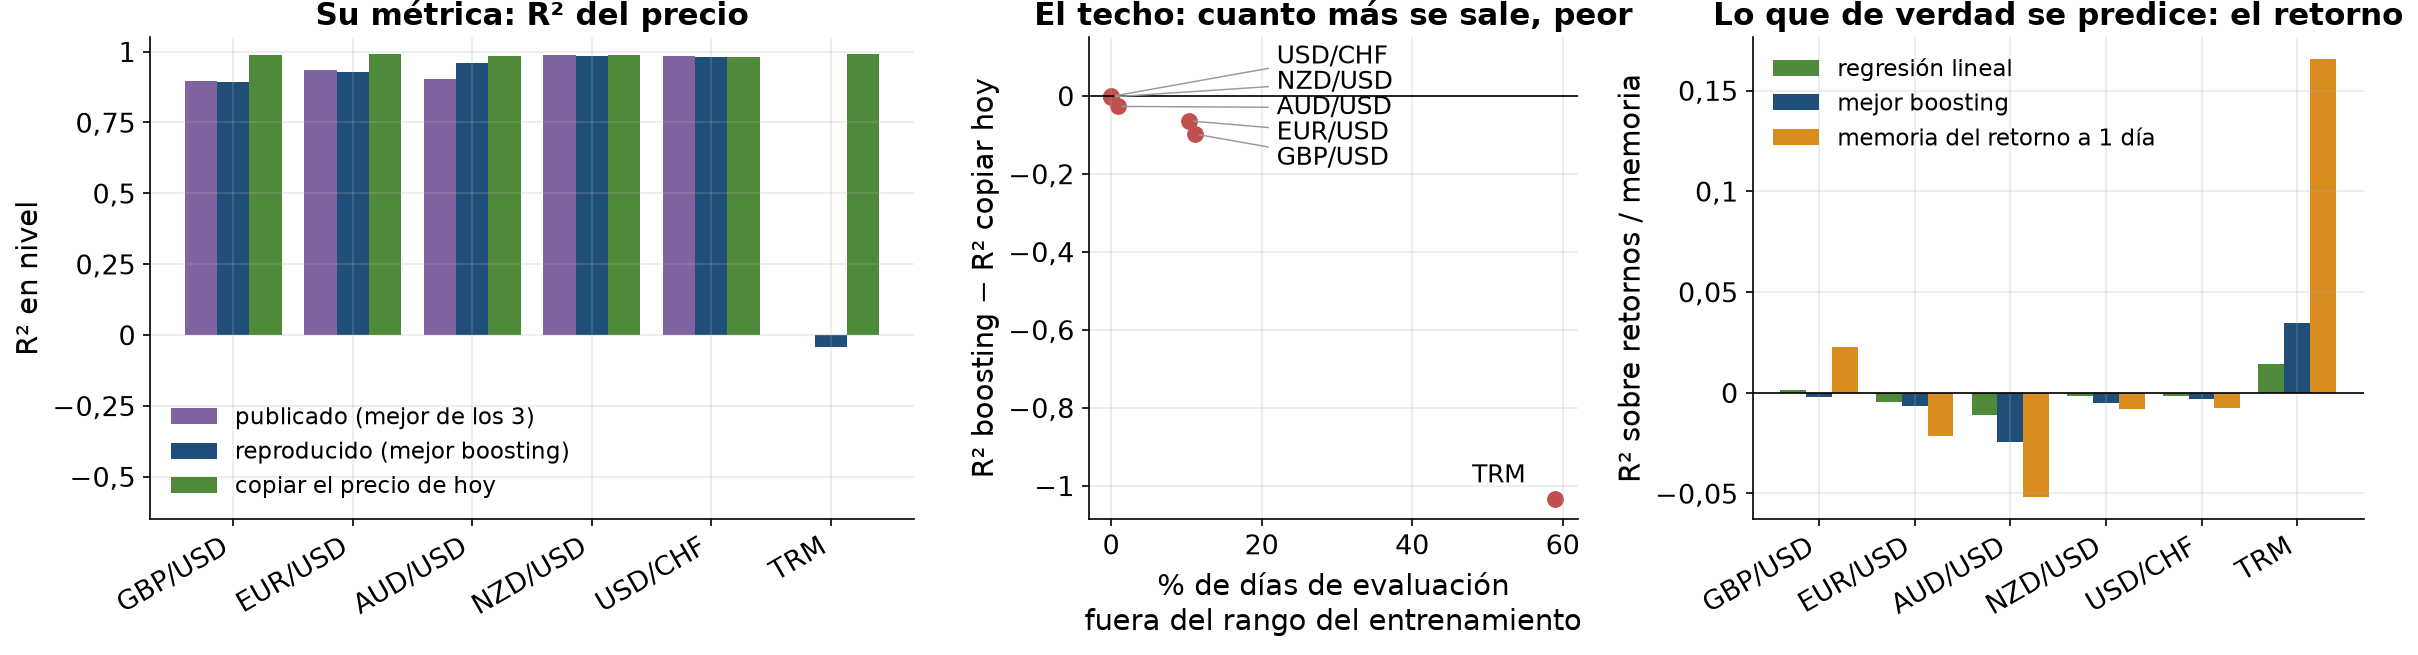
\includegraphics[width=\textwidth]{fig_articulo_vs_trm.png}
\caption{El método del artículo con sus propios datos y con la TRM. Izquierda: su $R^2$ en nivel (publicado y reproducido) no supera a copiar el precio de hoy. Centro: cuanto más se sale la evaluación del rango de entrenamiento, más pierden los árboles. Derecha: en retornos, la TRM es la única serie con algo de señal.}
\label{fig:articulo}
\end{figure}

\paragraph{Modelo final.} Elegimos CatBoost con solo la TRM con la regla que fijamos en la Entrega~2, antes de abrir el test: el boosting con menor error en validación, salvo que fuera significativamente peor que la base. No lo es: su diferencia con la lineal es de $-0{,}16$ pesos (intervalo de $-0{,}49$ a $+0{,}13$; $p=0{,}32$). Como los siete modelos quedan a centavos, la decisión no se apoya solo en ese número. Es estable: le gana a la base en cuatro de los cinco cortes y queda primero en validación y segundo en el test, a 0,01 pesos de la lineal, mientras que los modelos con macro caen al fondo. No usa macro, porque no aportan. Y es interpretable: tres variables, todas de la TRM, y un comportamiento que cabe en una curva (sección~4). Esa curva es también la razón para preferir un árbol a una recta: un salto grande no se repite en proporción, y el árbol aprende un tope que la recta no tiene. Lo decimos con todas las letras: empata con la regresión lineal, que es igual de válida y más simple; por eso la aplicación la muestra a su lado, y ese empate es parte de la respuesta. Su configuración es de profundidad 2, 200 árboles y tasa de aprendizaje 0,03; en el test tiene un RMSE de 35,64 pesos y un MAE de 27,09. Para la aplicación lo reentrenamos con los 5.401 días y los mismos hiperparámetros.

% -------------------------------------------------------------------------------------
\section*{4. Interpretación del modelo final}

Con SHAP (valores de Shapley, que reparten cada predicción entre las variables) \cite{shap} y dependencia parcial (Figura~\ref{fig:interpretacion}), el movimiento de hoy concentra el 82~\% de la importancia y empuja la predicción en su misma dirección; los de hace 5 y 10 publicaciones pesan poco, y las variables casi no interactúan (8~\% del efecto). El efecto tiene forma de S: el modelo repite cerca del 20~\% de un movimiento pequeño (la lineal, el 17~\%), pero con un tope de $+35$ puntos básicos al subir y $-24$ al bajar. Si hoy la TRM sube 3~\%, la lineal espera $+50$ puntos básicos y el modelo se queda en $+35$: un salto grande no se repite en proporción.

\begin{figure}[!htbp]
\centering
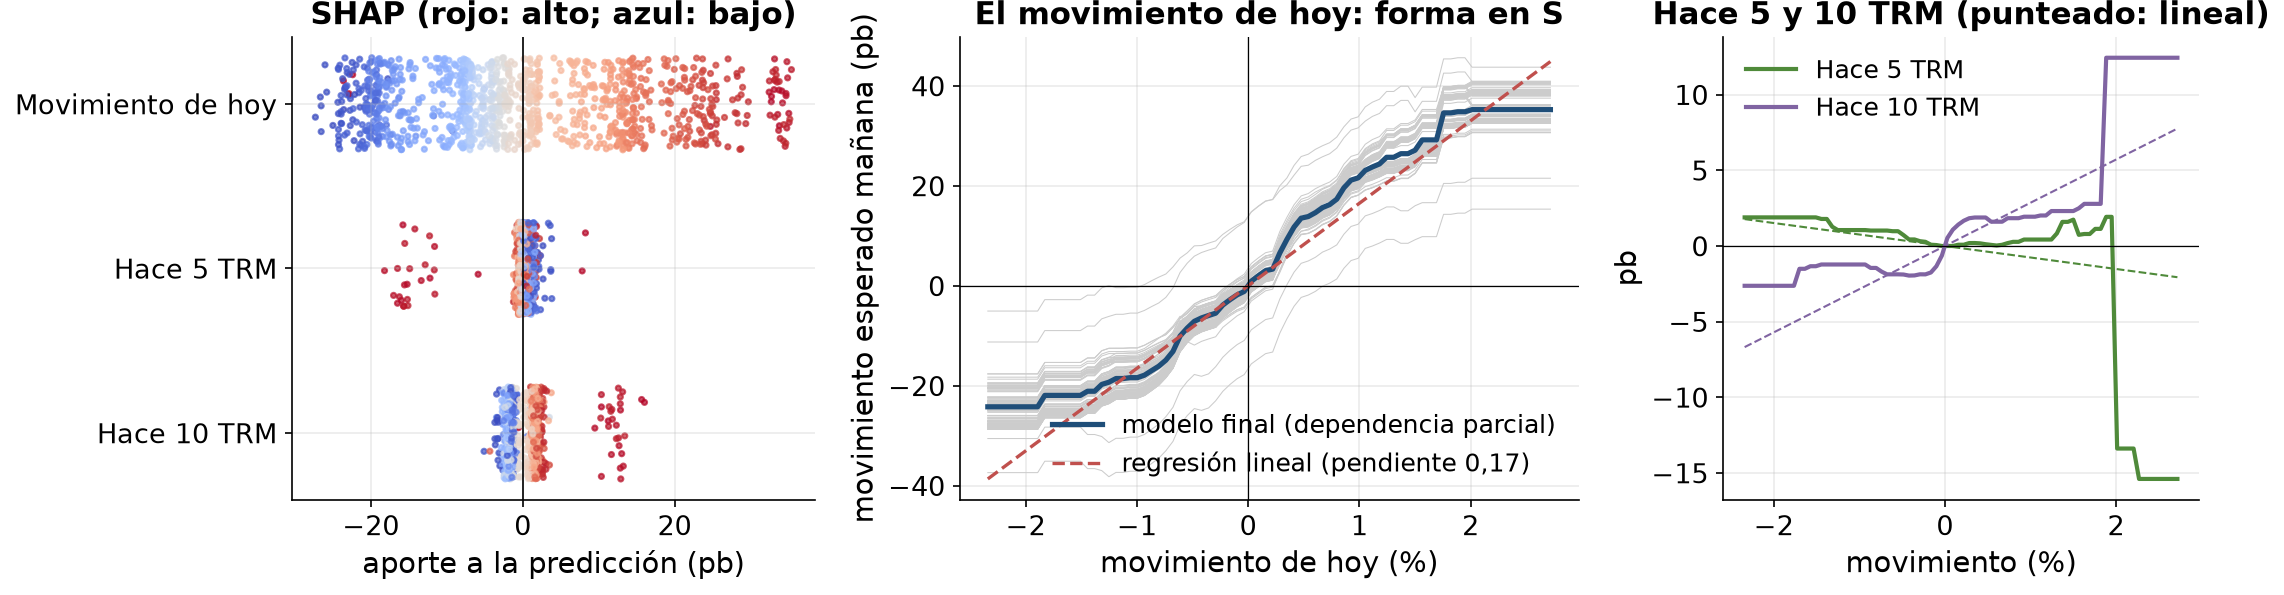
\includegraphics[width=\textwidth]{fig_interpretacion.png}
\caption{Qué mira el modelo final en el test. Izquierda: aporte SHAP de cada variable (cada punto es un día). Centro: dependencia parcial del movimiento de hoy frente a la recta de la regresión lineal. Derecha: los movimientos de hace 5 y 10 publicaciones.}
\label{fig:interpretacion}
\end{figure}

\paragraph{Un día concreto.} El 7 de octubre de 2023 la TRM era 4.386,66. El modelo partió de su valor medio (+0,8 puntos básicos) y sumó +13,7 por el movimiento de hoy (una subida de 0,62~\%), +9,5 por el de hace 10 publicaciones y $-15{,}5$ por el de hace 5, que habían sido subidas de más del 2~\%: predijo 4.390,35. La TRM fue 4.231,97, una caída de 3,5~\%; el error, de 158 pesos, es el peor del test (COP 15,8 millones para el importador), y la lineal falló casi igual (162 pesos). Ninguna variable anticipaba ese salto. La aplicación muestra este mismo desglose para cada predicción.

\paragraph{Tipos de error.} El modelo acierta si la TRM sube o baja el 55~\% de los días, casi lo mismo que decir siempre ``baja'' (54~\%; $p=0{,}16$): no sirve para elegir cuándo comprar dólares. El error lo deciden los días grandes: el 10~\% de días con movimientos más grandes produce la mitad del error cuadrático, y con el mercado agitado el error típico sube de 19 a 30 pesos. No hay sesgo (en promedio, $-0{,}7$ pesos). Frente a no usar modelo (``mañana igual que hoy''), el modelo reduce el error en 0,39 pesos por dólar: poco, pero real ($p=0{,}002$).

\begin{table}[!htbp]
\centering\footnotesize
\setlength{\tabcolsep}{4pt}
\caption{Error en el test para un importador que compra USD 100.000 (2022--2026).}
\label{tab:importador}
\begin{tabular}{lcccccc}
\toprule
 & \multicolumn{2}{c}{Error típico (MAE)} & \multicolumn{2}{c}{9 de cada 10 días, menor a} & \multicolumn{2}{c}{Peor día} \\
\cmidrule(lr){2-3}\cmidrule(lr){4-5}\cmidrule(lr){6-7}
Pronóstico & \$/USD & COP millones & \$/USD & COP millones & \$/USD & COP millones \\
\midrule
Modelo final & 27,09 & 2,7 & 55,70 & 5,6 & 158,38 & 15,8 \\
Regresión lineal & 27,10 & 2,7 & 55,70 & 5,6 & 162,03 & 16,2 \\
Mañana igual que hoy & 27,48 & 2,7 & 59,44 & 5,9 & 154,69 & 15,5 \\
\bottomrule
\end{tabular}

\end{table}

\paragraph{Qué significa.} Para un importador (Tabla~\ref{tab:importador}), el modelo es un valor de referencia para presupuestar el día siguiente y una medida del riesgo: el error típico en una compra de USD 100.000 es de COP 2,7 millones, y uno de cada diez días supera los COP 5,6 millones. No sirve para escoger el día de compra ni para planear con semanas de anticipación; para protegerse de los días grandes, la herramienta es una cobertura, no un pronóstico. Para el Banco de la República, el caso del diferencial muestra que su relación con la TRM depende del episodio, así que su efecto debe leerse en horizontes más largos. \textbf{Alcance:} la conclusión es predictiva y a un día, no causal; no dice que el petróleo o las tasas no afecten la TRM, sino que el dato de hoy no anticipa el movimiento de mañana.

% -------------------------------------------------------------------------------------
\section*{5. Despliegue}

La aplicación (Streamlit \cite{streamlit}) toma las últimas TRM publicadas en datos.gov.co, calcula las variables con las mismas funciones del proyecto, predice la próxima TRM con el modelo final y con la regresión lineal, y explica la predicción con SHAP (Figura~\ref{fig:app}). El usuario también puede elegir una fecha pasada, para ver qué habría predicho el modelo, o escribir a mano las últimas TRM. Si la fuente falla, usa la copia congelada y lo avisa. Un semáforo verifica la coherencia entre los datos de uso y los de entrenamiento: datos recientes, historia completa, valores dentro de lo visto, régimen de volatilidad y modelo correcto. Catorce pruebas automáticas comprueban, entre otras cosas, que las variables que calcula la aplicación son idénticas a las del entrenamiento en los 5.401 días y que sus predicciones coinciden con las del test. La aplicación está en \enlaceapp; el README de la carpeta \texttt{app} explica cómo ejecutarla.

\begin{figure}[!htbp]
\centering
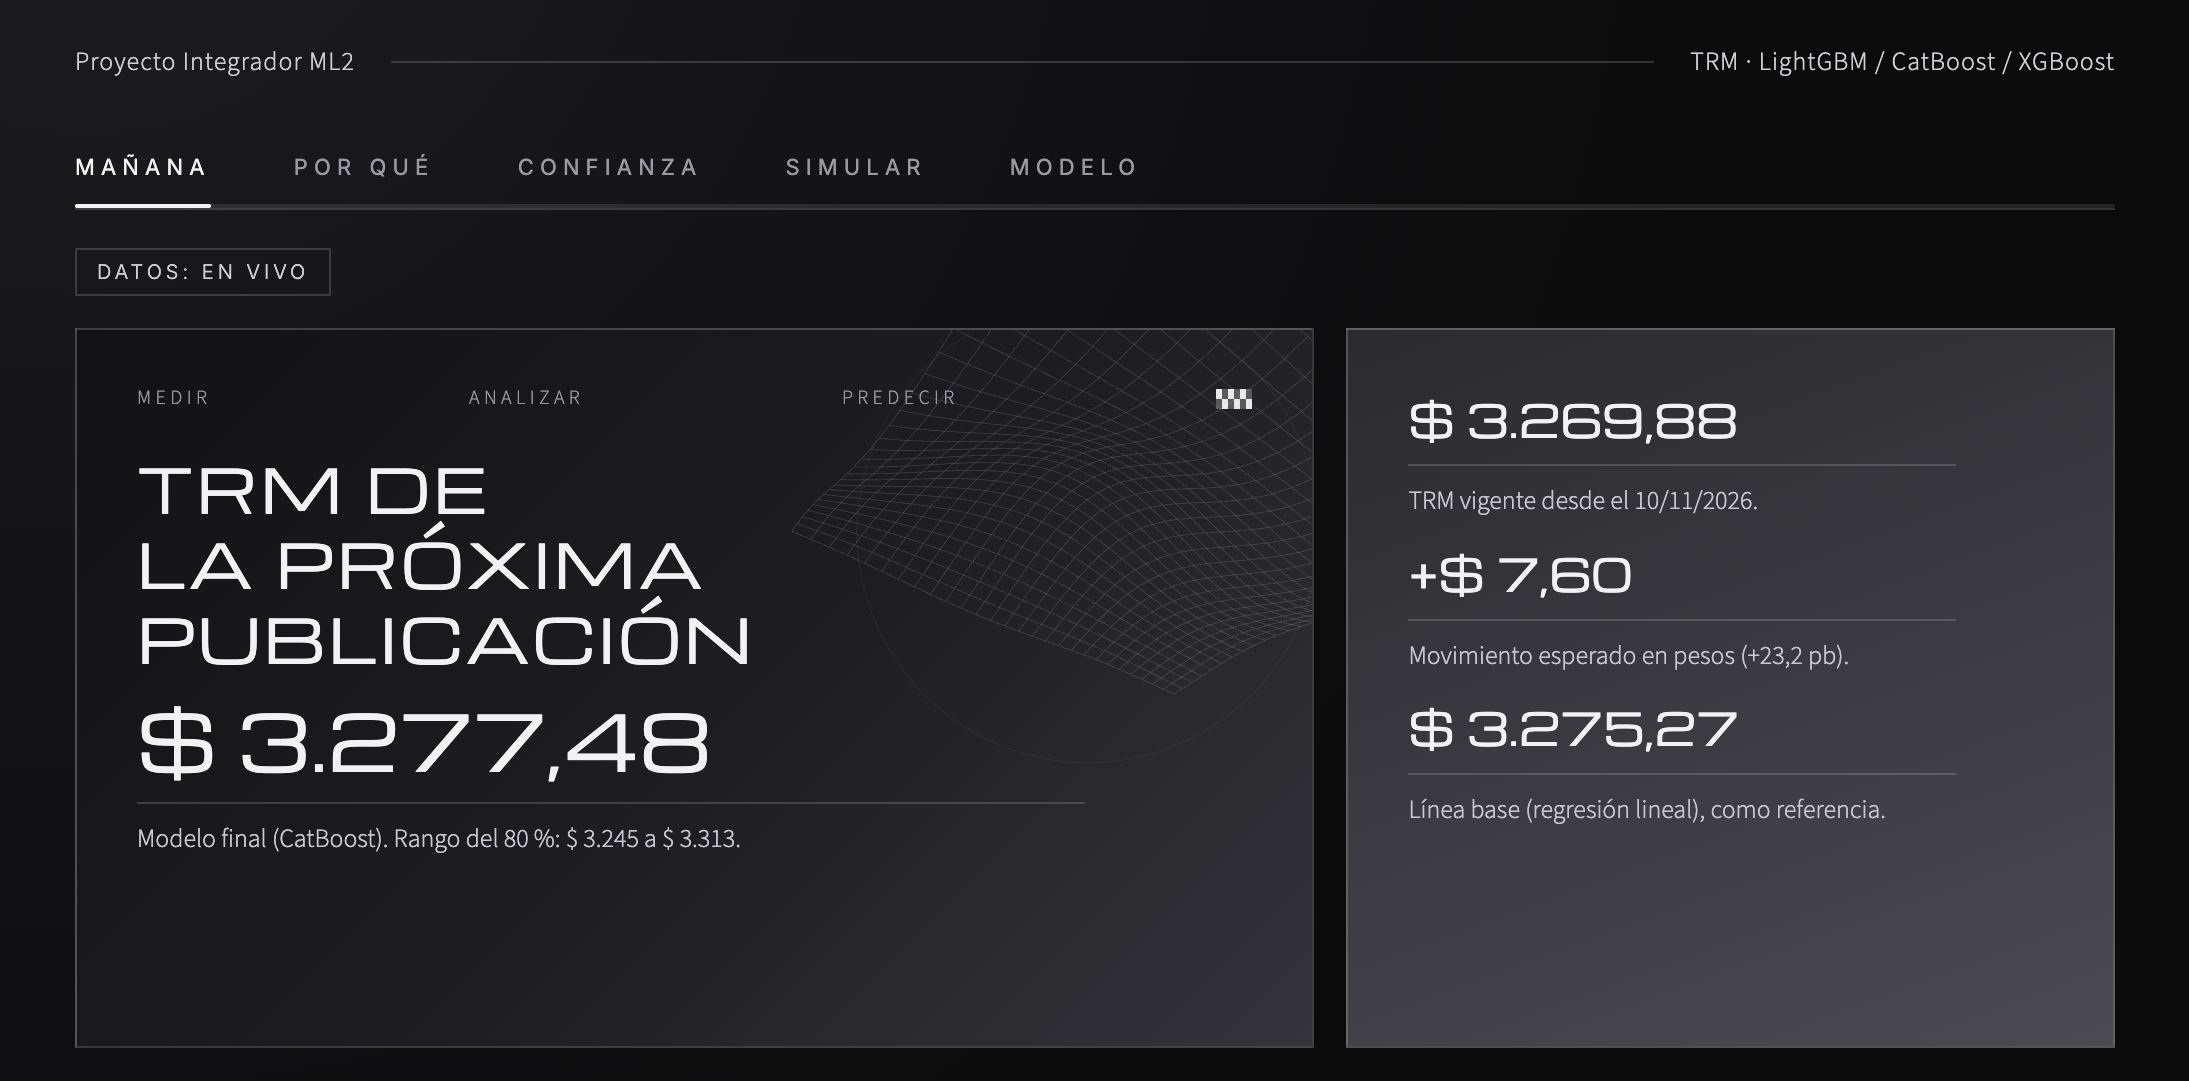
\includegraphics[width=0.82\textwidth]{fig_app.png}
\caption{La aplicación el 10 de noviembre de 2026, con datos en vivo: TRM vigente, próxima TRM según el modelo final y la línea base, y rango del 80~\%.}
\label{fig:app}
\end{figure}

% -------------------------------------------------------------------------------------
\section*{6. Limitaciones y proyección}

\begin{table}[!htbp]
\centering\footnotesize
\setlength{\tabcolsep}{4pt}
\renewcommand{\arraystretch}{0.95}
\caption{Limitaciones principales, con su evidencia y lo que se hizo.}
\label{tab:limitaciones}
\begin{tabular}{>{\raggedright\arraybackslash}p{2.3cm}>{\raggedright\arraybackslash}p{6.6cm}>{\raggedright\arraybackslash}p{6.3cm}}
\toprule
Categoría & Limitación y evidencia & Qué se hizo \\
\midrule
Datos & Solo las variables de la Entrega 1; el DXY no viene de una fuente oficial & Copia congelada con MD5; TRM verificada \\
Simulación & No hubo: datos reales, pero una sola historia; no se probaron escenarios que no ocurrieron & Cinco periodos de validación y un test con crisis y choques \\
Sobreajuste & El modelo con macro aprendió un régimen de un solo episodio & Validación anidada; árboles poco profundos; modelo final sin macro \\
Estabilidad & Diferencias de centavos; el orden de los modelos cambia entre validación y test & Pruebas formales; robustez con Optuna \\
Generalización & Un solo test, ya abierto en la Entrega 2; el rango fijo cubría solo el 67~\% de los días agitados & Elección solo con validación; rango adaptativo; datos nuevos \\
\bottomrule
\end{tabular}
\end{table}

La Tabla~\ref{tab:limitaciones} resume las limitaciones. Probamos dos mejoras que responden a las dos más fuertes. La primera es un rango de predicción que se ensancha con la volatilidad de las últimas 40 TRM (ventana elegida solo con la validación): en el test, la TRM real cae dentro del rango del 80~\% en el 80~\% de los días, frente al 71~\% del rango fijo (67~\% con el mercado agitado), y la aplicación ya lo usa (Figura~\ref{fig:rango}). La segunda es evaluar el modelo en 28 TRM publicadas después del test, que nunca vio: su error típico fue de 19,7 pesos, en empate con la lineal y con ``mañana igual que hoy'', y el rango contuvo la TRM real en 26 de los 28 días.

\begin{figure}[!htbp]
\centering
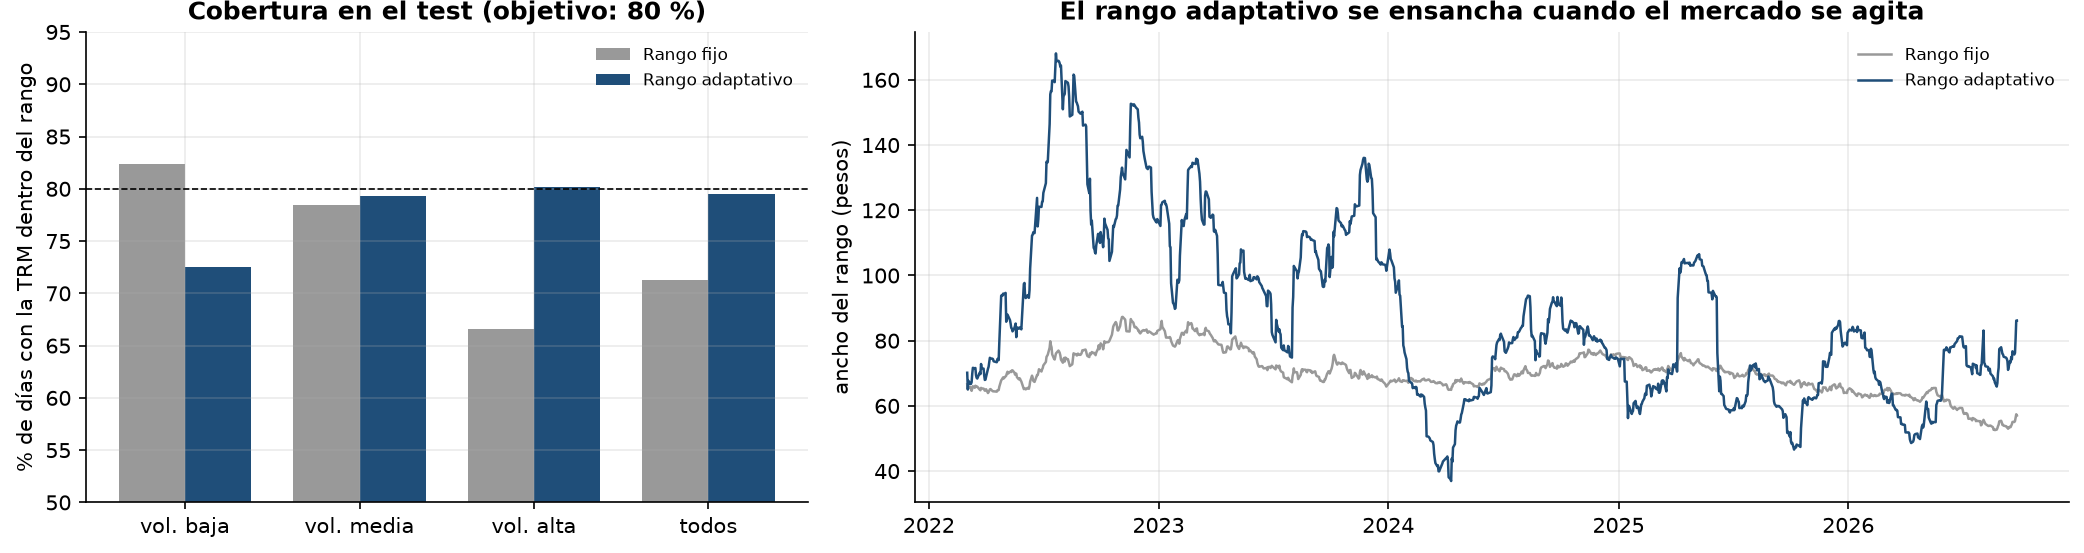
\includegraphics[width=0.92\textwidth]{fig_rango_adaptativo.png}
\caption{Rango del 80~\% fijo y adaptativo en el test. Izquierda: porcentaje de días con la TRM real dentro del rango, según la volatilidad. Derecha: el rango adaptativo se ensancha cuando el mercado se agita.}
\label{fig:rango}
\end{figure}

\paragraph{Proyección.} Las líneas de continuidad son agregar variables con información del mismo día (VIX, peso mexicano, intervenciones del Banrep), predecir el tamaño del movimiento en lugar de su dirección (que sí tiene memoria) y mirar horizontes de semanas. En \emph{Deep Learning}, los modelos de secuencias (LSTM, Temporal Fusion Transformer) y el pronóstico probabilístico (DeepAR) son el paso natural, con una expectativa honesta: con cerca del 3~\% de señal a un día, más complejidad no tiene qué aprender, salvo con datos intradía o más variables, y se evaluarían con el mismo protocolo. En \emph{MLOps}, el proyecto ya tiene datos y modelos versionados, validación de datos en uso, pruebas automáticas y despliegue; siguen la descarga programada, un registro de modelos, alertas de deriva, un reentrenamiento mensual que solo acepte un modelo nuevo si no es peor que el actual, y la ejecución automática de las pruebas en cada cambio.

% -------------------------------------------------------------------------------------
\section*{Conclusiones}

Las variables macroeconómicas no mejoran la predicción diaria de la TRM, y ningún gradient boosting le gana a una regresión lineal: lo único predecible es que mañana repite una pequeña parte del movimiento de hoy, con un tope. Esa memoria es real, pero vale unos 0,4 pesos por dólar frente a no usar modelo, no sirve para elegir el día de compra y no anticipa los saltos grandes. El alto $R^2$ del artículo no contradice este resultado: mide la persistencia del precio, no la capacidad de predecir.

% ===================== Final =====================
\begin{thebibliography}{99}
\small
\bibitem{articulo} Eslami Ghayour, A., \& Yousefi, A. (2023). \textit{Performance Analysis of Gradient Boosting Models for Forex Market Prediction}. SSRN. \url{https://ssrn.com/abstract=4450688}. Datos: \href{https://github.com/arasheslamii/1-Performance-comparison-of-Gradient-Boosting-algorithms-for-Forex-market-Prediction-A-Study-on-Lig}{repositorio del autor en GitHub (arasheslamii), commit 506912c}
\bibitem{banrep} Banco de la República de Colombia. \textit{Servicio web de estadísticas (SDMX): TRM y tasa de política monetaria}. \url{https://www.banrep.gov.co}
\bibitem{superfin} Superintendencia Financiera de Colombia. \textit{Tasa de Cambio Representativa del Mercado}. Datos Abiertos Colombia. \url{https://www.datos.gov.co}
\bibitem{fred} Federal Reserve Bank of St. Louis. \textit{Brent - Europe (DCOILBRENTEU) y Federal Funds Effective Rate (DFF)}. FRED. \url{https://fred.stlouisfed.org}
\bibitem{yahoo-dxy} Yahoo Finance. \textit{US Dollar Index (DX-Y.NYB)}. \url{https://finance.yahoo.com/quote/DX-Y.NYB}
\bibitem{lightgbm} Ke, G., et al. (2017). LightGBM: A Highly Efficient Gradient Boosting Decision Tree. \textit{Advances in Neural Information Processing Systems}, 30.
\bibitem{catboost} Prokhorenkova, L., et al. (2018). CatBoost: Unbiased Boosting with Categorical Features. \textit{Advances in Neural Information Processing Systems}, 31.
\bibitem{xgboost} Chen, T., \& Guestrin, C. (2016). XGBoost: A Scalable Tree Boosting System. \textit{Proceedings of the 22nd ACM SIGKDD Conference}, 785--794.
\bibitem{sklearn} Pedregosa, F., et al. (2011). Scikit-learn: Machine Learning in Python. \textit{Journal of Machine Learning Research}, 12, 2825--2830.
\bibitem{optuna} Akiba, T., et al. (2019). Optuna: A Next-generation Hyperparameter Optimization Framework. \textit{Proceedings of the 25th ACM SIGKDD Conference}, 2623--2631.
\bibitem{dm} Diebold, F. X., \& Mariano, R. S. (1995). Comparing Predictive Accuracy. \textit{Journal of Business \& Economic Statistics}, 13(3), 253--263.
\bibitem{nw} Newey, W. K., \& West, K. D. (1987). A Simple, Positive Semi-Definite, Heteroskedasticity and Autocorrelation Consistent Covariance Matrix. \textit{Econometrica}, 55(3), 703--708.
\bibitem{hln} Harvey, D., Leybourne, S., \& Newbold, P. (1997). Testing the Equality of Prediction Mean Squared Errors. \textit{International Journal of Forecasting}, 13(2), 281--291.
\bibitem{shap} Lundberg, S. M., \& Lee, S.-I. (2017). A Unified Approach to Interpreting Model Predictions. \textit{Advances in Neural Information Processing Systems}, 30.
\bibitem{streamlit} Streamlit (2026). \textit{Streamlit: A faster way to build and share data apps}. \url{https://streamlit.io}
\end{thebibliography}

\paragraph{Código.} Repositorio del proyecto, carpeta \texttt{Entrega 2}: datos congelados, código documentado, notebooks 01 a 10 (el README indica la instalación y el orden de ejecución), aplicación y pruebas:\\
\url{https://github.com/Gatitomalo1234/Proyecto-Machine-Learning-2}

\paragraph{Uso de IA.} Usamos Claude (Anthropic), a través de Claude Code, como asistente para estructurar y documentar el código, revisar la metodología frente a la rúbrica, construir la aplicación y redactar borradores. Las decisiones y la interpretación son nuestras, y cada cifra de este informe sale de las salidas del código.

\end{document}
